\documentclass[11pt,a4paper]{article}

    \usepackage[utf8x]{inputenc}
    \usepackage{graphicx}
    \usepackage[english]{babel}
    \usepackage{color}
    \usepackage{fontspec}
    \usepackage{float}
    \usepackage{caption}
    \usepackage{subcaption}
    \usepackage{mathtools}
    \usepackage{algorithm2e}
    \usepackage{enumerate}
    \usepackage{diagbox}
    \usepackage{multirow}

    \usepackage{pythonhighlight} % python

    \usepackage{color}
    \definecolor{dkgreen}{rgb}{0,0.6,0}
    \definecolor{gray}{rgb}{0.5,0.5,0.5}
    \definecolor{mauve}{rgb}{0.58,0,0.82}
    \definecolor{dark}{rgb}{0.1,0.2,0.5}

    \lstset{frame=tb,
    language=Python,
    aboveskip=3mm,
    belowskip=3mm,
    showstringspaces=false,
    columns=flexible,
    basicstyle={\small\ttfamily},
    numbers=left,
    numberstyle=\tiny\color{gray},
    keywordstyle=\color{blue},
    commentstyle=\color{dkgreen},
    stringstyle=\color{mauve},
    breaklines=true,
    frame=single,
    breakatwhitespace=true,
    tabsize=3
    }
    
    \usepackage{hyperref} % the option is there to remove the square around links which is what I don't like.
    \hypersetup{
    colorlinks = true,
    linkcolor = dark,
    filecolor = blue,
    citecolor = black,      
    urlcolor = cyan,
    }
    \usepackage{perpage} 
    \MakePerPage{footnote} % Reset the footnote counter perpage. may require to run latex twice.
    
    \usepackage[margin=2cm]{geometry} % This is here to fit more text into the page.
    
  %  \setcounter{secnumdepth}{1}  % This removes the numbering from the subsections.
                            % If you want the numbering of the subsection level just remove this line
    
    \title{\textsc{COMP7405 - Assignment 3}}
    \author{	3035562069 YAN Qiangyu\\
                ZENG Jiaxing \\
                WANG Kai
            }
    \date{}
    
    \setlength{\parindent}{0pt} % No indentation for paragraphs. Because that is just old.
    \setlength{\parskip}{\baselineskip} % Instead use vertical paragraph spacing.
    
    \fontencoding{T1} % the better font encoding.
    
    %\setmainfont{Helvetical} % Setting the main font here. But I like the default font alot so this is commented out.
    
    \begin{document}
    \maketitle

    \section{Interface Introduction}
    
    \begin{figure}[h]
    \centering
    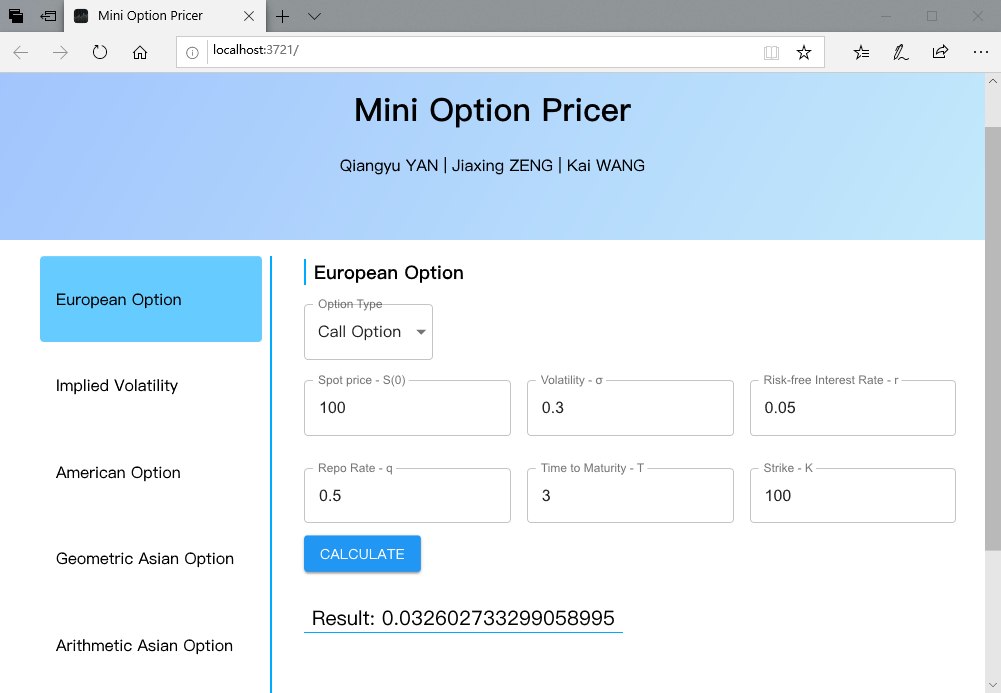
\includegraphics[width=\linewidth]{snapshot1}
    \caption{UI SnapShot}
    \end{figure}

    The User Interface is developed using 
    \emph{Flask} (A python web framework) 
    and \emph{HTML} \& \emph{CSS} \& \emph{JavaScript}. 
    It's a webpage.
    

    Look at the snapshot above. There is a menu on the left panel which can
    be click and navigate to different option pricer calculator. On the
    right panel, it provides several input fields, such as Option Type, Spot
    Price and so on.

    After filling in these input fields, we can click on the button
    "CALCULATE" and the result will be displayed below.

    \newpage
    \section{Functionalities Explanation}
    \begin{verbatim}
    .                               # For more details, please refer to source code.
    |-- option_pricer
    |   |-- binomial_tree.py        # American options
    |   |-- black_scholes.py        # European options
    |   |-- closed_form_formulas.py # Geometric Asian/Basket options
    |   |-- implied_volatility.py   # Implied volatility calculator
    |   |-- MC.py                   # Monte Carlo Method (Arithmetic Asian/Basket option)
    |   |-- server.py               # HTTP Server
    |   |-- static                  # Web User Interface compiled file directory
    |-- README.md
    |-- requirement.txt             # Python Dependencies
    |-- web                         # Web User Interface source code
    \end{verbatim}

    


    \section{Test cases and analysis} 

    Form previous knowledges, we know that 
    the correlation of the variates and values 
    may not be monotance, 
    so all the analysis only based on the testing
    result, which means it may variates
    under different conditions.
    
    \begin{table}[h]
        \caption{European Option}
        \centering
        \scalebox{0.82}{
        \begin{tabular}{|c|c|c|c|c|c|c|c|c|}
            \hline
            No. &$S(0)$ & $K$ & $T$ & $q$
            & $\sigma$ & $r$ & Call & Put\\
            \hline
            0  & 100 & 100 & 3 & 0.2 & 0.3 & 0.05
            & 3.7385 & 34.9281 \\
            \hline
            1+ & \textbf{120} & 100 & 3 & 0.2 & 0.3 & 0.05 
            & 7.4270 & 27.6404 \\
            \hline
            1- & \textbf{80} & 100 & 3 & 0.2 & 0.3 & 0.05 
            & 1.4346 & 43.6004 \\
            \hline
            2+ & 100 & \textbf{120} & 3 & 0.2 & 0.3 & 0.05 
            & 2.0720 & 50.4758 \\
            \hline
            2- & 100 & \textbf{80} & 3 & 0.2 & 0.3 & 0.05 
            & 6.8517 & 20.8272 \\
            \hline
            3+ & 100 & 100 & \textbf{4} & 0.2 & 0.3 & 0.05 
            & 2.9468 & 39.8870 \\
            \hline
            3- & 100 & 100 & \textbf{2} & 0.2 & 0.3 & 0.05 
            & 4.6054 & 28.0571 \\
            \hline
            4+ & 100 & 100 & 3 & \textbf{0.3} & 0.3 & 0.05 
            & 0.9993 & 46.4131 \\
            \hline
            4- & 100 & 100 & 3 & \textbf{0.1} & 0.3 & 0.05 
            & 11.0827 & 23.0717 \\
            \hline
            5+ & 100 & 100 & 3 & 0.2 & \textbf{0.4} & 0.05
            & 7.2639 & 38.3535 \\
            \hline
            5- & 100 & 100 & 3 & 0.2 & \textbf{0.2} & 0.05
            & 1.0750 & 32.2646 \\
            \hline
            6+ & 100 & 100 & 3 & 0.2 & 0.3 & \textbf{0.10}
            & 5.6942 & 24.8948 \\
            \hline
            6- & 100 & 100 & 3 & 0.2 & 0.3 & \textbf{0.03}
            & 3.1088 & 39.6207 \\
            \hline
        \end{tabular}
        }
    \end{table}

    From \hyperref[T1]{Table 1}, 
    we can get: Based on Case 0,
    (1) Call Option value will increase(decrease) when 
    $ S(0) / \sigma / r$ increase(decrease), or
    $ K / T / q$ decrease/increase; 
    (2) Put Option value will increase(decrease) when
    $ K / T / q / \sigma $ increase(decrease), or
    $ S(0) / r$ decrease(increase).





    \newpage
    \begin{table}[h]
        \label{T2}
        \caption{Implied Volatility}
        \centering
        \scalebox{0.82}{
        \begin{tabular}{|c|c|c|c|c|c|c|c|c|}
            \hline
            No. & Price & $S(0)$ & $K$ & 
            $T$ & $q$ & $r$ & $\sigma_C$ & $\sigma_P$ \\
            \hline
            0 & 25 & 100 & 100 & 1 & 0.2 & 0.05 
            & 0.9158 & 0.5044 \\
            \hline
            1+ & \textbf{27} & 100 & 100 & 1 & 0.2 & 0.05 
            & 0.9801 & 0.5656 \\
            \hline
            1- & \textbf{23} & 100 & 100 & 1 & 0.2 & 0.05 
            & 0.8522 & 0.4429 \\
            \hline
            2+ & 25 & \textbf{120} & 100 & 1 & 0.2 & 0.05 
            & 0.6164 & 0.7021\\
            \hline
            2- & 25 & \textbf{90} & 100 & 1 & 0.2 & 0.05 
            & 1.0863 & 0.3346 \\
            \hline
            3+ & 25 & 100 & \textbf{110} & 1 & 0.2 & 0.05 
            & 0.9904 & 0.2608 \\
            \hline
            3- & 25 & 100 & \textbf{90} & 1 & 0.2 & 0.05 
            & 0.8260 & 0.7054 \\
            \hline
            4+ & 25 & 100 & 80 & \textbf{2} & 0.2 & 0.05 
            & 0.8541 & 0.1970 \\
            \hline
            4- & 25 & 100 & 80 & \textbf{0.5} & 0.2 & 0.05 
            & 1.0978 & 0.8143 \\
            \hline
            5+ & 25 & 100 & 100 & 1 & \textbf{0.3} & 0.05 
            & 1.0775 & 0.3460 \\
            \hline
            5- & 25 & 100 & 100 & 1 & \textbf{0.1} & 0.05 
            & 0.7538 & 0.6205 \\
            \hline
            6+ & 25 & 100 & 100 & 1 & 0.2 & \textbf{0.07} 
            & 0.8994 & 0.5448 \\
            \hline
            6- & 25 & 100 & 100 & 1 & 0.2 & \textbf{0.03} 
            & 0.9319 & 0.4620 \\
            \hline
    \end{tabular}
        }
    \end{table}


    (need to revise)From Table 2, 
    we can get: Based on Case 0,
    (1) Call Option value will increase(decrease) when 
    $ S(0) / \sigma / r$ increase(decrease), or
    $ K / T / q$ decrease/increase; 
    (2) Put Option value will increase(decrease) when
    $ K / T / q / \sigma $ increase(decrease), or
    $ S(0) / r$ decrease(increase).















    \begin{table}[h]
        \label{T3}
        \caption{American Option}
        \centering
        \scalebox{0.82}{
        \begin{tabular}{|c|c|c|c|c|c|c|c|c|}
            \hline
            No. &$S(0)$ & $K$ & $T$ &
            $\sigma$ & $r$ & $N$ & Call & Put\\
            \hline
            0  & 100 & 100 & 3 & 0.3 & 0.05 & 5 
            & 27.6113 & 15.2564 \\
            \hline
            1+ & \textbf{120} & 100 & 3 & 0.3 & 0.05 & 5 
            & 41.9701 & 9.1557 \\
            \hline
            1- & \textbf{80} & 100 & 3 & 0.3 & 0.05 & 5 
            & 13.2526 & 23.8372 \\
            \hline
            2+ & 100 & \textbf{120} & 3 & 0.3 & 0.05 & 5 
            & 18.7749 & 26.2878 \\
            \hline
            2- & 100 & \textbf{80} & 3 & 0.3 & 0.05 & 5 
            & 36.4478 & 6.1963 \\
            \hline
            3+ & 100 & 100 & \textbf{4} & 0.3 & 0.05 & 5 
            & 32.4964 & 16.4948 \\
            \hline
            3- & 100 & 100 & \textbf{2} & 0.3 & 0.05 & 5 
            & 21.9150 & 13.3923 \\
            \hline
            4+ & 100 & 100 & 3 & \textbf{0.4} & 0.05 & 5 
            & 33.8292 & 21.6133 \\
            \hline
            4- & 100 & 100 & 3 & \textbf{0.2} & 0.05 & 5 
            & 21.3850 & 8.7914 \\
            \hline
            5+ & 100 & 100 & 3 & 0.3 & \textbf{0.10} & 5 
            & 34.0587 & 10.9048 \\
            \hline
            5- & 100 & 100 & 3 & 0.3 & \textbf{0.03} & 5 
            & 25.1147 & 17.3811 \\
            \hline
            6+ & 100 & 100 & 3 & 0.3 & 0.05 & \textbf{7} 
            & 27.3803 & 11.0762 \\
            \hline
            6- & 100 & 100 & 3 & 0.3 & 0.05 & \textbf{3} 
            & 28.1473 & 15.2788 \\
            \hline
    \end{tabular}
        }
    \end{table}


    From \hyperref[T3]{Table 3}, we can get: Based on Case 0,
    (1) Call Option value will increase(decrease) when 
    $ S(0) / T / \sigma / r / N$ increase(decrease), or
    $ K $ decrease/increase; 
    (2) Put Option value will increase(decrease) when
    $ K / T / \sigma $ increase(decrease), or
    $ S(0) / r / N$ decrease(increase).

    \begin{figure}[htbp]
        \centering
        \begin{minipage}[t]{0.48\textwidth}
        \centering
        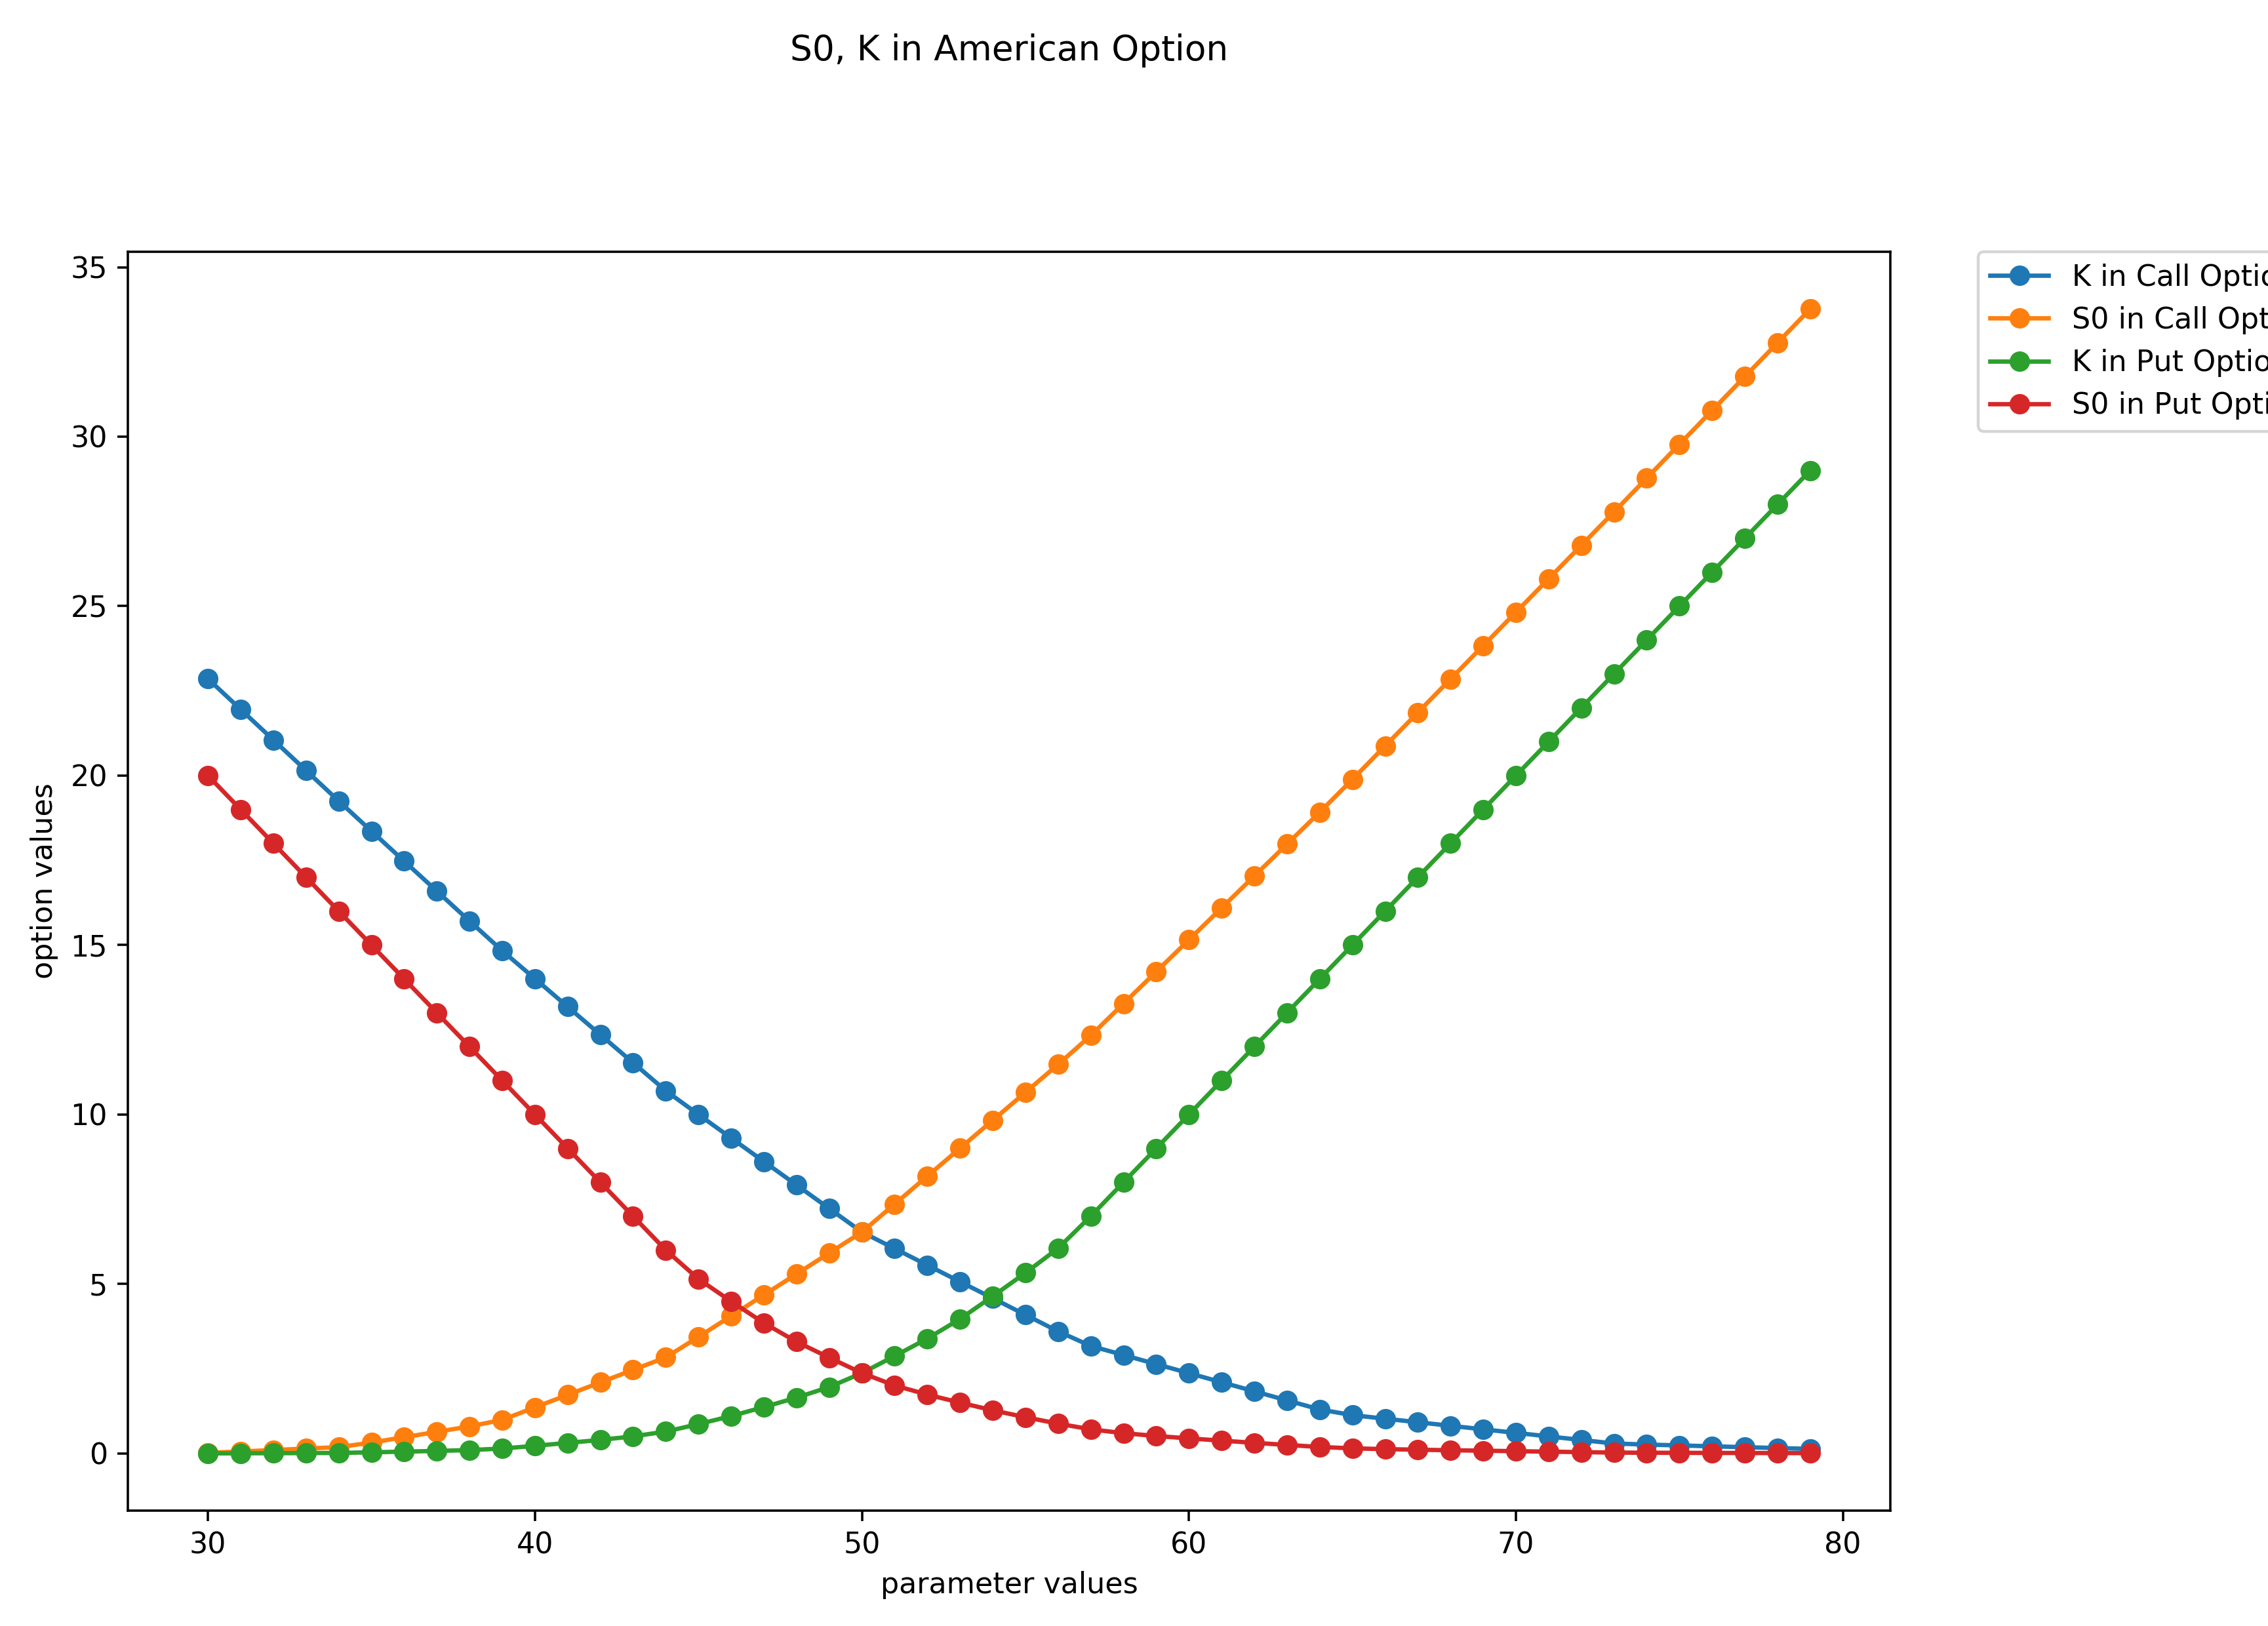
\includegraphics[width=7.5cm]{S0KAO}
        \end{minipage}
        \begin{minipage}[t]{0.48\textwidth}
        \centering
        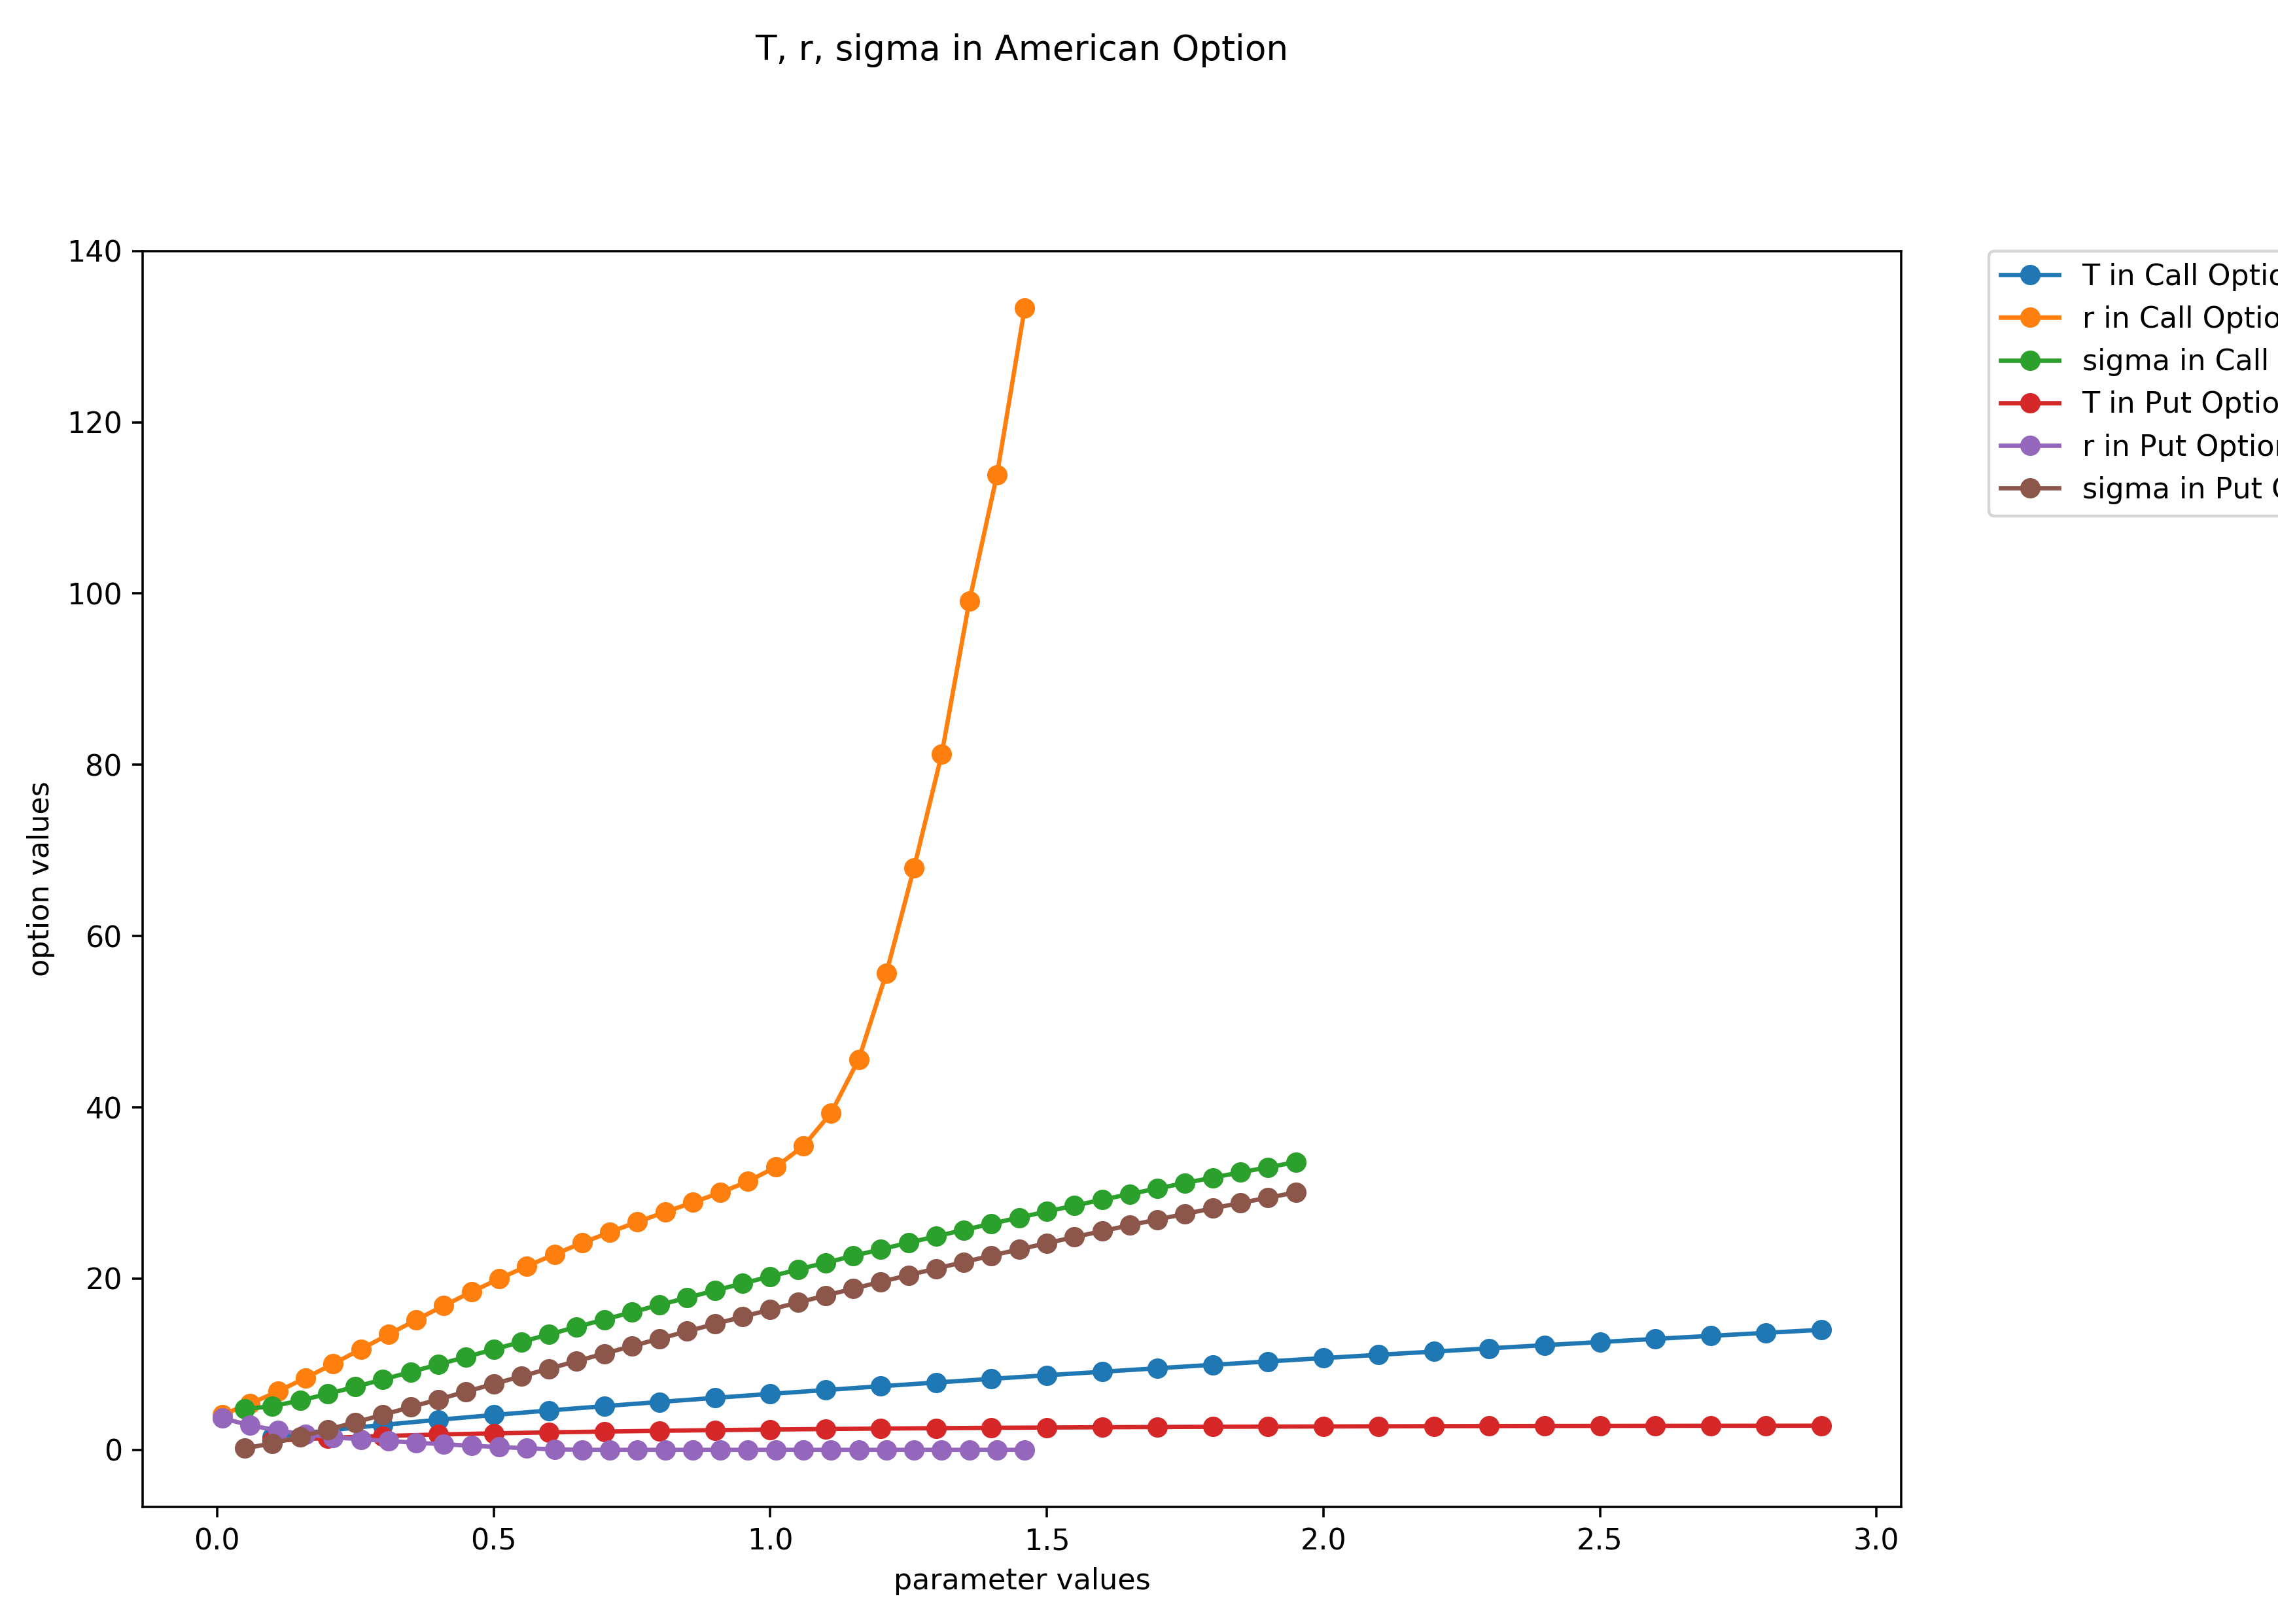
\includegraphics[width=7.5cm]{TrsigmaAO}
        \end{minipage}
    \end{figure}


    For more information, we crate the chart to represent
    the relationship.
    Based on $K=50, r=0.1, \sigma=0.2, S(0)=50$, 
    and the step of binomial tree is 10,
    we test $K$ from 30 to 80, $S(0)$ from 30 to 80, 
    $T$ from 0.1 to 3, $r$ from 0.01 to 1.5, 
    $\sigma$ from 0,05 to 2. 



    \newpage
    \begin{table}[htbp]
        \label{T4}
        \caption{Geometric Asian Option}
        \centering
        \scalebox{0.69}{
        \begin{tabular}{|c|c|c|c|c|c|c|c|c|}
            \hline
            Test No. &$S(0)$ & $K$ & $T$ &
            $\sigma$ & $r$ & $n$ & Call & Put\\
            \hline
            0 & 100 & 100 & 3 & 0.3 & 0.05 & 50
            &  &  \\
            \hline
            1+ & \textbf{120} & 100 & 3 & 0.3 & 0.05 & 50
            &  &  \\
            \hline
            1- & \textbf{80} & 100 & 3 & 0.3 & 0.05 & 50
            &  &  \\
            \hline
            2+ & 100 & \textbf{120} & 3 & 0.3 & 0.05 & 50
            &  &  \\
            \hline
            2- & 100 & \textbf{80} & 3 & 0.3 & 0.05 & 50
            &  &  \\
            \hline
            3+ & 100 & 100 & \textbf{4} & 0.3 & 0.05 & 50
            &  &  \\
            \hline
            3- & 100 & 100 & \textbf{2} & 0.3 & 0.05 & 50
            &  &  \\
            \hline
            4+ & 100 & 100 & 3 & \textbf{0.4} & 0.05 & 50
            &  &  \\
            \hline
            4- & 100 & 100 & 3 & \textbf{0.2} & 0.05 & 50
            &  &  \\
            \hline
            5+ & 100 & 100 & 3 & 0.3 & \textbf{0.10} & 50
            &  &  \\
            \hline
            5- & 100 & 100 & 3 & 0.3 & \textbf{0.03} & 50
            &  &  \\
            \hline
            6+ & 100 & 100 & 3 & 0.3 & 0.05 & \textbf{100}
            &  &  \\
            \hline
            6- & 100 & 100 & 3 & 0.3 & 0.05 & \textbf{30}
            &  &  \\
            \hline
    \end{tabular}
        }
    \end{table}

    
    (need to revise)From \hyperref[T4]{Table 4}, we can get: Based on Case 0,
    (1) Call Option value will increase(decrease) when 
    $ S(0) /  T / \sigma / r$ increase(decrease), or
    $ K$ decrease/increase; 
    (2) Put Option value will increase(decrease) when
    $ K / T / \sigma $ increase(decrease), or
    $ S(0) / r$ decrease(increase);
    (3) $n$ usually won't affect the option value a lot.



    \begin{table}[h]
        \label{T5}
        \caption{Arithmetric Option}
        \centering
        \scalebox{0.69}{
        \begin{tabular}{|c|c|c|c|c|c|c|c|c|c|c|c|}
            \hline
            No. &$S(0)$ & $K$ & $T$ &
            $\sigma$ & $r$ & $n$ & $m(k)$ & $Call_0$ & $Put_0$ 
            & $Call_1$ & $Put_1$ \\
            \hline
            0  & 100 & 100 & 3 & 0.3 & 0.05 & 50 & 100
            & [14.5328, 14.8193] & [7.7782, 7.9165] 
            & [14.7196, 14.7412] & [7.8024, 7.8112]\\
            \hline
            0* & 100 & 100 & 3 & 0.3 & 0.05 & 50 & 100
            & [14.6382, 14.9257] & [7.6845, 7.8224] 
            & [14.7232, 14.7450] & [7.7949, 7.8038]\\
            \hline
            1+ & \textbf{120} & 100 & 3 & 0.3 & 0.05 & 50 & 100
            & [28.4026, 28.8034] & [3.1498, 3.2390] 
            & [28.6764, 28.7044] & [3.1634, 3.1719]\\
            \hline
            1- & \textbf{80} & 100 & 3 & 0.3 & 0.05 & 50 & 100
            & [5.0763, 5.2405] & [16.8179, 17.0013] 
            & [5.1948, 5.2107] & [16.8699, 16.8796]\\
            \hline
            2+ & 100 & \textbf{120} & 3 & 0.3 & 0.05 & 50 & 100 
            & [7.5411, 7,7620] & [17.9305, 18.1435] 
            & [7.6950, 7.7152] & [17.9870, 17.9983]\\
            \hline
            2- & 100 & \textbf{80} & 3 & 0.3 & 0.05 & 50 & 100 
            & [25.8763, 26.2178] & [1.9273, 2.0356] 
            & [26.1147, 26.1284] & [1.9846, 1.9913]\\
            \hline
            3+ & 100 & 100 & \textbf{4} & 0.3 & 0.05 & 50 & 100 
            & [16.9239, 17.2637] & [8.1950, 8.3406] 
            & [17.1441, 17.1746] & [8.2193, 8.2300]\\
            \hline
            3- & 100 & 100 & \textbf{2} & 0.3 & 0.05 & 50 & 100 
            & [11.6636, 11.8892] & [7.0222, 7.1473] 
            & [11.8116, 11.8251] & [7.0453, 7.0518]\\
            \hline
            4+ & 100 & 100 & 3 & \textbf{0.4} & 0.05 & 50 & 100 
            & [17.9294, 18.3309] & [11.2506, 11.4307] 
            & [18.1931, 18.2340] & [11.2855, 11.3010]\\
            \hline
            4- & 100 & 100 & 3 & \textbf{0.2} & 0.05 & 50 & 100 
            & [11.1576, 11.3450] & [4.3411, 4.4312] 
            & [11.2811, 11.2906] & [4.3569, 4.3607]\\
            \hline
            5+ & 100 & 100 & 3 & 0.3 & \textbf{0.10} & 50 & 100 
            & [17.2140, 17.5077] & [4.8335, 4.9367] 
            & [17.4057, 17.4299] & [4.8492, 4.8557]\\
            \hline
            5- & 100 & 100 & 3 & 0.3 & \textbf{0.03} & 50 & 100 
            & [13.4598, 13.7419] & [9.3022, 9.4564] 
            & [13.6463, 13.6669] & [9.3326, 9.3425]\\
            \hline
            6+ & 100 & 100 & 3 & 0.3 & 0.05 & \textbf{100} & 100
            & [14.5575, 14.8447] & [7.6720, 7.8094] 
            & [14.5923, 15.6135] & [7.7473, 7.7561]\\
            \hline
            6- & 100 & 100 & 3 & 0.3 & 0.05 & \textbf{30} & 100
            & [14.5566, 14.8441] & [7.8557, 7.9952] 
            & [14.8895, 14.9119] & [7.8707, 7.8797]\\
            \hline
    \end{tabular}
        }
        \footnotesize

    Default random seed is 10. 
    Case $0^*$ is using 5 as random seed.

    $Call_0$ and $Put_0$ are the result without control,
    $Call_1$ and $Put_1$ are the result with control variate.
    \end{table}

    From \hyperref[T5]{Table 5}, we can get: Based on Case 0,
    (1) Call Option value will increase(decrease) when 
    $ S(0) /  T / \sigma / r$ increase(decrease), or
    $ K$ decrease/increase; 
    (2) Put Option value will increase(decrease) when
    $ K / T / \sigma $ increase(decrease), or
    $ S(0) / r$ decrease(increase);
    (3) $n$ usually won't affect the option value a lot.

    




    \begin{table}[h]
        \label{T6}
        \caption{Geometric Asian Basket}
        \centering
        \scalebox{0.69}{
        \begin{tabular}{|c|c|c|c|c|c|c|c|c|c|c|c|}
            \hline
            No. &$S_1(0)$  &$S_2(0)$ & $K$ & $T$ &
            $\sigma_1$ & $\sigma_2$& $r$ & $\rho$ &
            Call & Put \\
            \hline
            0  & 100 & 100 & 100 & 3 & 0.3 & 0.3 & 0.05 & 0.5 & 22.1021 & 11.4916
            \\
            \hline
            1+ & \textbf{120} & \textbf{120} & 100 & 3 & 0.3 & 0.3 & 0.05 & 0.5 & 36.6832 & 6.7364
            \\
            \hline
            1- & \textbf{80} & \textbf{80} & 100 & 3 & 0.3 & 0.3 & 0.05 & 0.5 & 10.5840 & 19.3097
            \\
            \hline
            2+ & 100 & 100 & \textbf{120} & 3 & 0.3 & 0.3 & 0.05 & 0.5 & 14.6855 & 21.2891
            \\
            \hline
            2- & 100 & 100 & \textbf{80} & 3 & 0.3 & 0.3 & 0.05 & 0.5 & 32.5363 & 4.7116
            \\
            \hline
            3+ & 100 & 100 & 100 & \textbf{4} & 0.3 & 0.3 & 0.05 & 0.5 & 25.8367 & 12.1100
            \\
            \hline
            3- & 100 & 100 & 100 & \textbf{2} & 0.3 & 0.3 & 0.05 & 0.5 & 17.6665 & 10.3751
            \\
            \hline
            4+ & 100 & 100 & 100 & 3 & \textbf{0.5} & \textbf{0.5} & 0.05 & 0.5 & 28.4494 & 23.4691
            \\
            \hline
            4--& 100 & 100 & 100 & 3 & \textbf{0.1} & \textbf{0.1} & 0.05 & 0.5 & 14.7662 & 1.2113
            \\
            \hline
            4- & 100 & 100 & 100 & 3 & \textbf{0.1} & 0.3 & 0.05 & 0.5 & 17.9247 & 6.5864
            \\
            \hline
            5+ & 100 & 100 & 100 & 3 & 0.3 & 0.3 & \textbf{0.10} & 0.5 & 29.0230 & 6.4235
            \\
            \hline
            5- & 100 & 100 & 100 & 3 & 0.3 & 0.3 & \textbf{0.03} & 0.5 & 19.5131 & 14.2249
            \\
            \hline
            6+ & 100 & 100 & 100 & 3 & 0.3 & 0.3 & 0.05 & \textbf{0.9} & 25.8788 & 12.6224
            \\
            \hline
            6- & 100 & 100 & 100 & 3 & 0.3 & 0.3 & 0.05 & \textbf{0.3} & 20.1535 & 10.8394
            \\
            \hline
    \end{tabular}
        }
    \end{table}

    ()From \hyperref[T6]{Table 6}, we can get: Based on Case 0,
    (1) Call Option value will increase(decrease) when 
    $ S(0) /  T / \sigma / r$ increase(decrease), or
    $ K$ decrease/increase; 
    (2) Put Option value will increase(decrease) when
    $ K / T / \sigma $ increase(decrease), or
    $ S(0) / r$ decrease(increase);
    (3) $n$ usually won't affect the option value a lot.




    \newpage
    \begin{table}[h]
        \label{T7}
        \caption{Arithmetric Asian Basket}
        \centering
        \scalebox{0.69}{
        \begin{tabular}{|c|c|c|c|c|c|c|c|c|c|c|c|c|c|c|}
            \hline
            No. &$S_1(0)$  &$S_2(0)$ & $K$ & $T$ &
            $\sigma_1$ & $\sigma_2$& $r$ & $\rho$ &
            $m(k)$ & $Call_0$ & $Put_0$ & $Call_1$ & $Put_1$\\
            \hline
            0  & 100 & 100 & 100 & 3 & 0.3 & 0.3 & 0.05 & 0.5 
            & 100 
            & [24.1454, 24.6262] & [10.5387, 10.7284] 
            & [24.4580, 24.5200] & [10.5670, 10.5913]\\
            \hline
            0* & 100 & 100 & 100 & 3 & 0.3 & 0.3 & 0.05 & 0.5 
            & 100 
            & [24.4490, 24.9341] & [10.4730, 10.6621]
            & [24.4576, 24.5201] & [10.5659, 10.5902]\\
            \hline
            1+ & \textbf{120} & \textbf{120} & 100 & 3 & 0.3 & 0.3 & 0.05 & 0.5 
            & 100 
            & [39.5611, 40.1950] & [6.0868, 6.2355] 
            & [39.9785, 40.0551] & [6.1012, 6.1212]\\
            \hline
            1- & \textbf{80} & \textbf{80} & 100 & 3 & 0.3 & 0.3 & 0.05 & 0.5 
            & 100 
            & [11.7723, 12.0930] & [18.0303, 18.2597]
            & [11.9840, 12.0300] & [18.0785, 18.1061]\\
            \hline
            2+ & 100 & 100 & \textbf{120} & 3 & 0.3 & 0.3 & 0.05 & 0.5 
            & 100 
            & [16.2783, 16.6952] & [19.8146, 20.0828]
            & [16.5535, 16.6121] & [19.8698, 19.9024]\\
            \hline
            2- & 100 & 100 & \textbf{80} & 3 & 0.3 & 0.3 & 0.05 & 0.5 
            & 100 
            & [34.9971, 35.5335] & [4.2431, 4.3546]
            & [35.3517, 35.4157] & [4.2524, 4.2676]\\
            \hline
            3+ & 100 & 100 & 100 & \textbf{4} & 0.3 & 0.3 & 0.05 & 0.5 
            & 100 
            & [28.7083, 29.2935] & [10.9846, 11.1824] 
            & [29.0876, 29.1743] & [11.0139, 11.0426]\\
            \hline
            3- & 100 & 100 & 100 & \textbf{2} & 0.3 & 0.3 & 0.05 & 0.5 
            & 100 
            & [18.9245, 19.2925] & [9.6463, 9.8201] 
            & [19.1646, 19.2037] & [9.6725, 9.6910]\\
            \hline
            4+ & 100 & 100 & 100 & 3 & \textbf{0.5} & \textbf{0.5} & 0.05 & 0.5 
            & 100
            & [34.2764, 35.2139] & [21.0047, 21,2980]
            & [34.8770, 35.0872] & [21.0632, 21.1196]\\
            \hline
            4--& 100 & 100 & 100 & 3 & \textbf{0.1} & \textbf{0.1} & 0.05 & 0.5 
            & 100
            & [14.9704, 15.1371] & [1.1592, 1.2010]
            & [15.0839, 15.0903] & [1.1596, 1.1619]\\
            \hline
            4- & 100 & 100 & 100 & 3 & \textbf{0.1} & 0.3 & 0.05 & 0.5 
            & 100
            & [19.1806, 19.5245] & [5.4966, 5.6117]
            & [19.4154, 19.4533] & [5.5160, 5.5331]\\
            \hline
            5+ & 100 & 100 & 100 & 3 & 0.3 & 0.3 & \textbf{0.10} & 0.5 
            & 100
            & [31.3679, 31.8890] & [5.8200, 5.9544] 
            & [31.7094, 31.7730] & [5.8338, 5.8517]\\
            \hline
            5- & 100 & 100 & 100 & 3 & 0.3 & 0.3 & \textbf{0.03} & 0.5 
            & 100
            & [21.4166, 21.8780] & [13.1101, 13.3245]
            & [21.7161, 21.7771] & [13.1454, 13.1724]\\
            \hline
            6+ & 100 & 100 & 100 & 3 & 0.3 & 0.3 & 0.05 & \textbf{0.9}
            & 100
            & [25.9909, 26.5407] & [12.3960, 12.6073]
            & [26.3479, 26.3605] & [12.4286, 12.4340]\\
            \hline
            6- & 100 & 100 & 100 & 3 & 0.3 & 0.3 & 0.05 & \textbf{0.3}
            & 100
            & [23.1861, 23.6333] & [9.5634, 9.7409]
            & [23.4685, 23.5544] & [9.5887, 9.6203]\\
            \hline
    \end{tabular}
        }
    \end{table}

    Default random seed is 10. 
    \texttt{0*} is using 5 as random seed.
    $Call_0$ and $Put_0$ are the result without control,
    $Call_1$ and $Put_1$ are the result with control variate.

    From \hyperref[T7]{Table 7}, we can see: Based on Case 0, 
    (1)Call Option value increases(decreases) if
    $ S_1(0)\&S_2(0) /  T $ 
    $/ \sigma_1 \& \sigma_2 / r / \rho$ 
    increase(decrease), or $ K$ decrease(increase); 
    (2)Put Option value increases(decreases) when
    $ K / T / \sigma_1\&\sigma_2$ 
    $ / \rho$ increases(decreases), 
    or $ S_1(0)\&S_2(0) / r$ decreases(increases).




    \section{Contributions}
    \begin{table}[h]
    \centering
    \begin{tabular}{|c|c|c|c|}
        \hline
        Task & YAN Qiangyu & ZENG Jiaxing & WANG Kai \\
        \hline
        European Option & & $\surd$ & \\
        \hline
        Implied Volatility && $\surd$ & \\
        \hline
        American Option &&& $\surd$ \\
        \hline
        Geometric Asian Option &&& $\surd$ \\
        \hline
        Arithmetric Asian Option & $\surd$ && \\
        \hline
        Geometric basket Option &&& $\surd$ \\
        \hline
        Arithmetric basket Option & $\surd$ && \\
        \hline
        UI Design && $\surd$ & \\
        \hline
        Test & $\surd$ & &  \\
        \hline
        Report & $\surd$ & $\surd$ &  \\
        \hline
    \end{tabular}
    \end{table}

    \end{document}